\documentclass[12pt]{article}
\usepackage[utf8]{inputenc}
\usepackage{graphicx}
\usepackage[hidelinks]{hyperref}
\usepackage{geometry}
\usepackage{url}
\geometry{a4paper, margin=1in}

\title{Java 2D\&3D Graphics Project2}
\author{m5271506 Kiyohiro Murai}
\date{2023-2-2}

\begin{document}

\maketitle
\tableofcontents
\newpage

\section{Classes}
Please see code for details. Here it will be written an overview of each class.
\subsection{ViewerMain.java}
A class with a main method. Has a JFrame. It composes the UI used by users.
\subsection{ViewerPanel.java}
A panel for displaying 3D models. The root object, Behavior, and Light are set.
If user specify the file path and view mode, the specified 3D shape will be
displayed.

\subsection{MeshManager.java}
Handles vertices, triangles, and graphs based on the triangle information in
the obj file. Calculates the shortest path between vertices and normal vectors.

\subsection{Face.java}
Class that handles triangular meshes
\subsection{Vector.java}
Class that handles vertices
\subsection{Dijkstra.java}
A class that uses Dijkstra's method to find the shortest path
\subsection{Graph.java}
Graph class used when searching for the shortest path
\subsection{PointCloud.java}
Class that displays PointCloud. When a vertex is selected, it has a method that
calculates the geodesic distance.
\subsection{WireFrame.java}
Class that displays WireFrame
\subsection{FilledWireFrame.java}
Class that displays FilledWireFrame
\subsection{FlatShading.java}
Class that displays FlatShading
\subsection{SmoothShading.java}
Class that displays SmoothShading. When a vertex is selected, it has a method
that calculates the geodesic distance.
\subsection{ColorMap.java}
Class that handles colormaps
\subsection{ColorMapManager.java}
A class that imports and manages colormaps from csv
\subsection{ObjReader.java}
Class that reads obj files

\section{FlatShading algorithm}
FlatShading.java performs flat shading of the input shape. First create a
triangle mesh using TriangleArray. Next, specify the normal vector for each
vertex of the triangle. Normal vector specifies the normal vector of the
triangular mesh.
\subsection{Normal vector of Mesh calculation}
The calculateFaceNormal(Vector v1, Vector v2, Vector v3) method of the
MeshManager class uses the given triangle
vertex coordinates to calculate the vectors of the two edges of the triangle.
Each edge vector is computed as a difference in vertex coordinates. Compute the
cross product of edge vectors edge1 and edge2 to obtain the normal vector of
the triangle. This normal vector indicates the orientation of the triangle's
surface.

\section{SmoothShading algorithm}
SmoothShading.java creates smooth sharding of 3D shapes. First, create a
triangle mesh using TriangleArray. Next, specify a normal vector for each
vertex.
\subsection{Normal vector of Vertices calculation}
Calculate the normal vector of the vertex using the calculateVerticesNorlmal()
method of the MeshManager class. The normal vector of each vertex is the
average value of the normal vectors of
neighboring meshes.

\section{Geodesic Distance algorithm}

\subsection{For data with triangle mesh information}
A graph was constructed based on the information about the edges of the
triangular mesh. Starting from the vertex selected by the user, the shortest
path to all other vertices is calculated using Dijkstra's algorithm. The
distance between vertices is calculated based on Euclidean distance. Since all
vertices are assigned a distance from the starting point, a color is set from
the color map based on that.
\subsection{For PointCloud with only vertex information}
A graph was created based on the k-nearest neighbor algorithm. As the number of
vertices increases, the amount of calculation increases and it takes more time.
With the test data provided, it took a huge amount of time to run.

\section{Problems}
\subsection{For PointCloud with only vertex information}
The k-nearest neighbor algorithm took an enormous amount of time to run on the
test data provided.
The use of kd tree can be considered for improvement. But I couldn't implement
it.

\subsection{Mouse translation problem}
I wanted to use the mouse to move a shape in translation, but for some reason
the
behavior didn't work properly. The officially stated default key (shift key)
was assigned a rotation function, but the movement function did not work
correctly.

\section{Screenshots}
\begin{figure}[h]
    \centering
    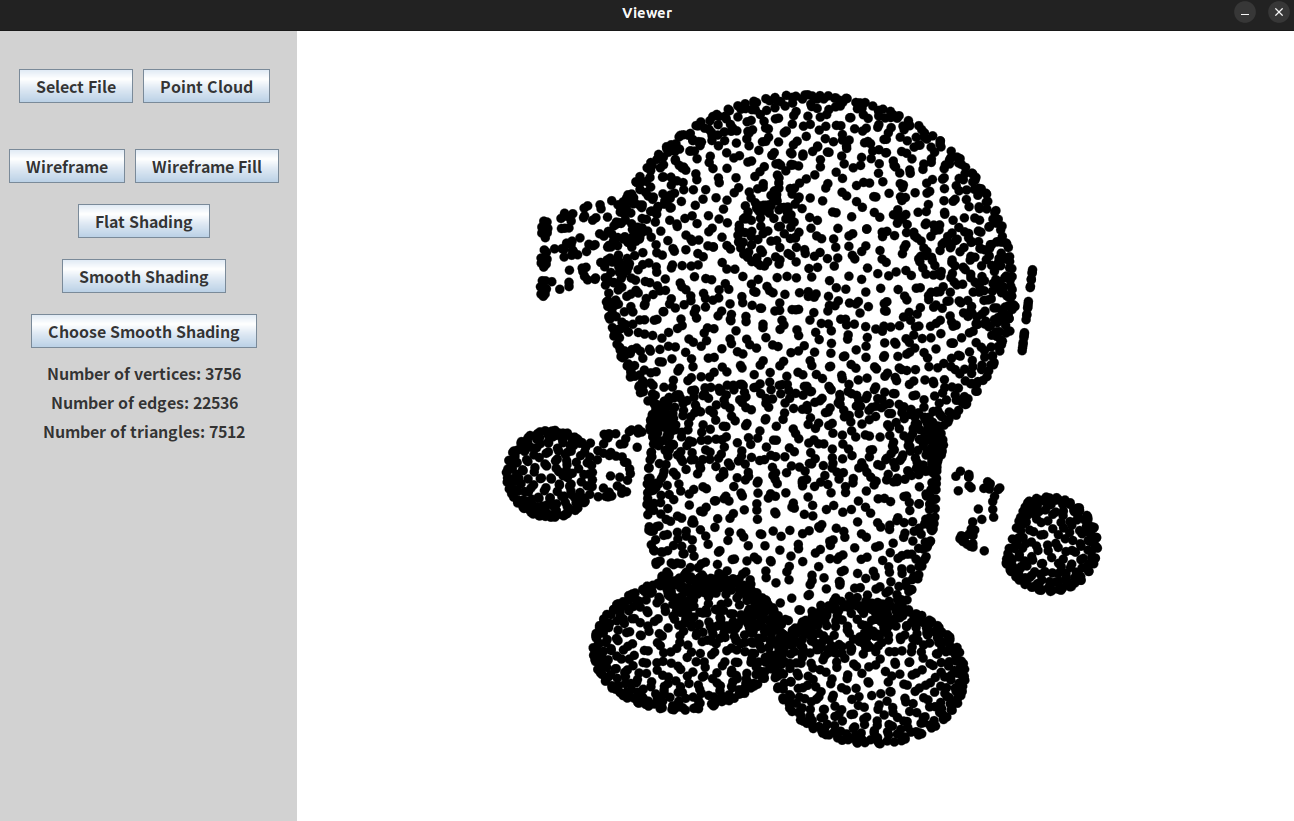
\includegraphics[width=1.0\textwidth]{sc1.png}
    \caption{Screenshot of PointCloud}
    \label{fig:my_label}
\end{figure}

\begin{figure}[h]
    \centering
    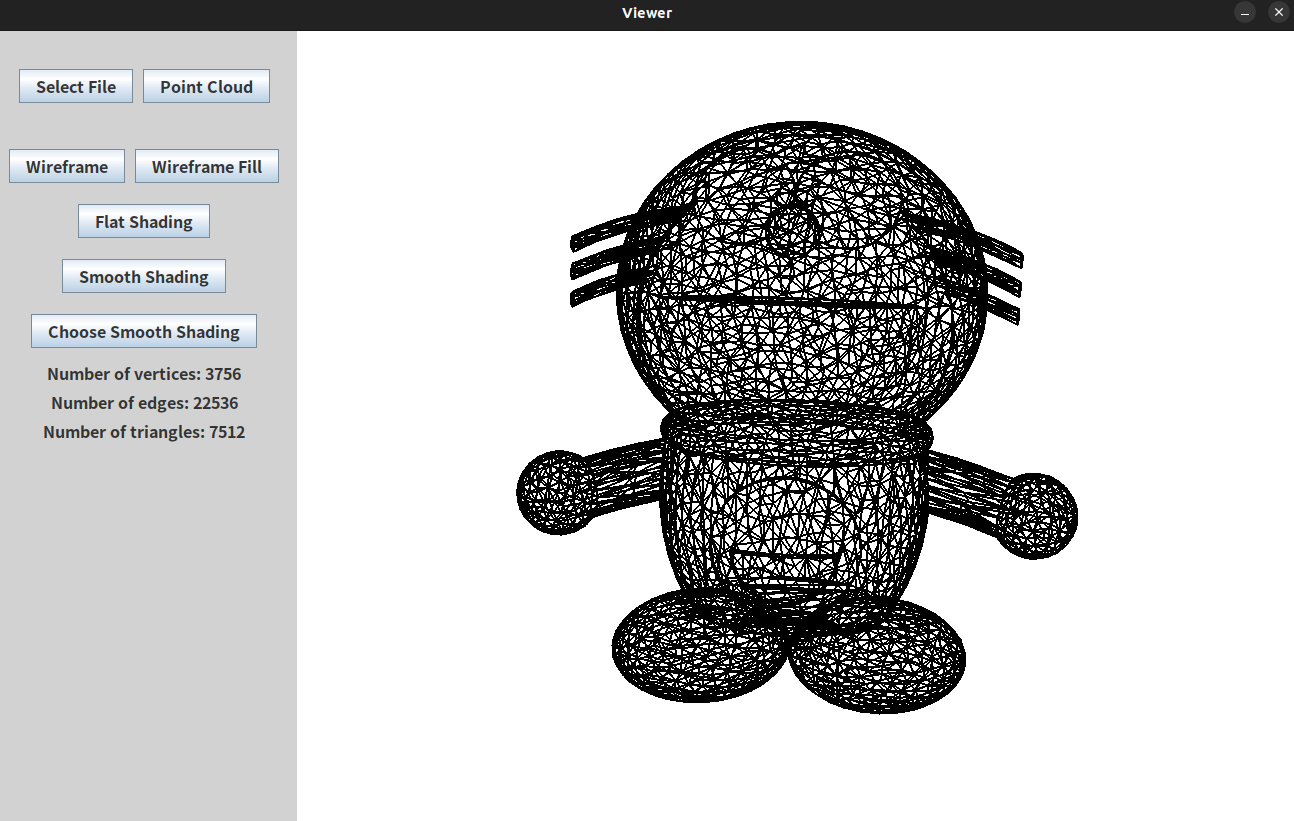
\includegraphics[width=1.0\textwidth]{sc2.png}
    \caption{Screenshot of WireFrame}
    \label{fig:my_label}
\end{figure}

\begin{figure}[h]
    \centering
    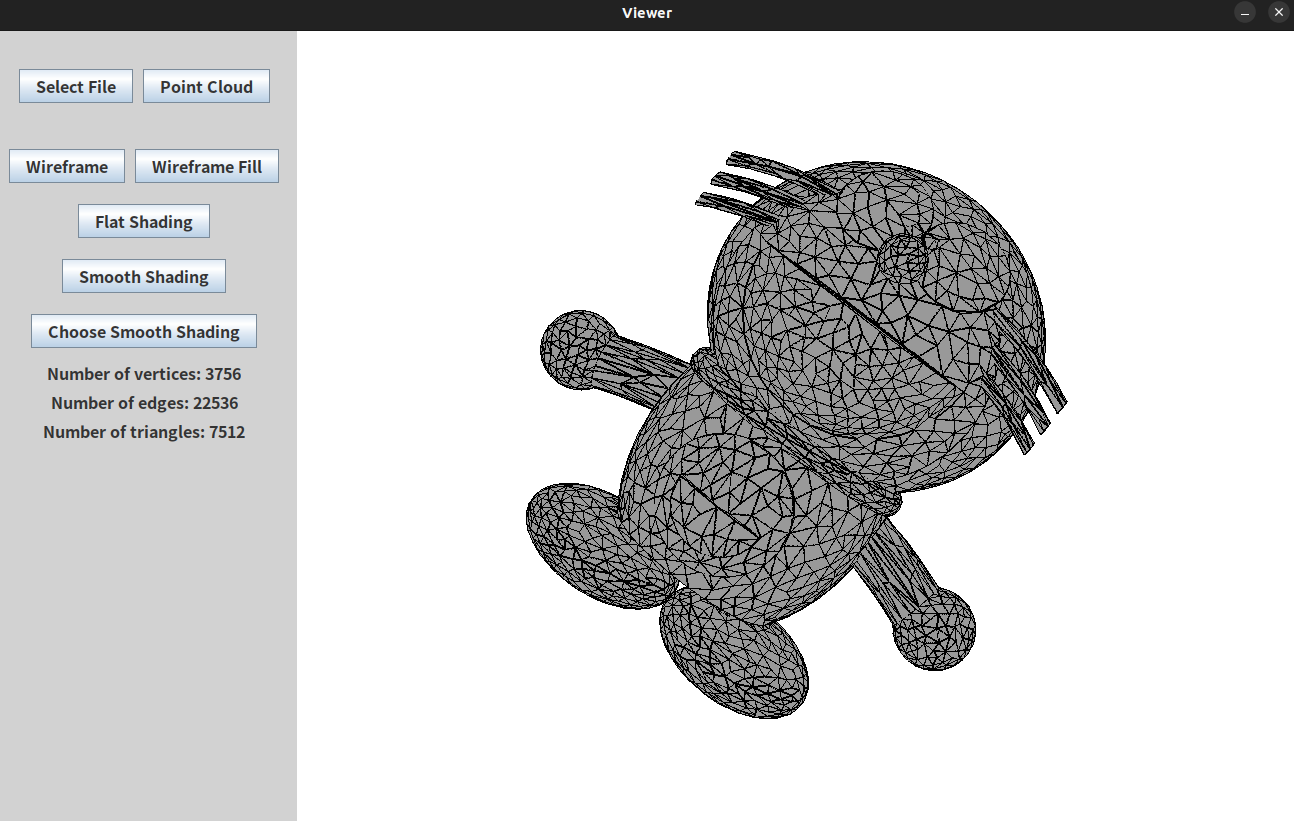
\includegraphics[width=1.0\textwidth]{sc3.png}
    \caption{Screenshot of FilledWireFrame}
    \label{fig:my_label}
\end{figure}

\begin{figure}[h]
    \centering
    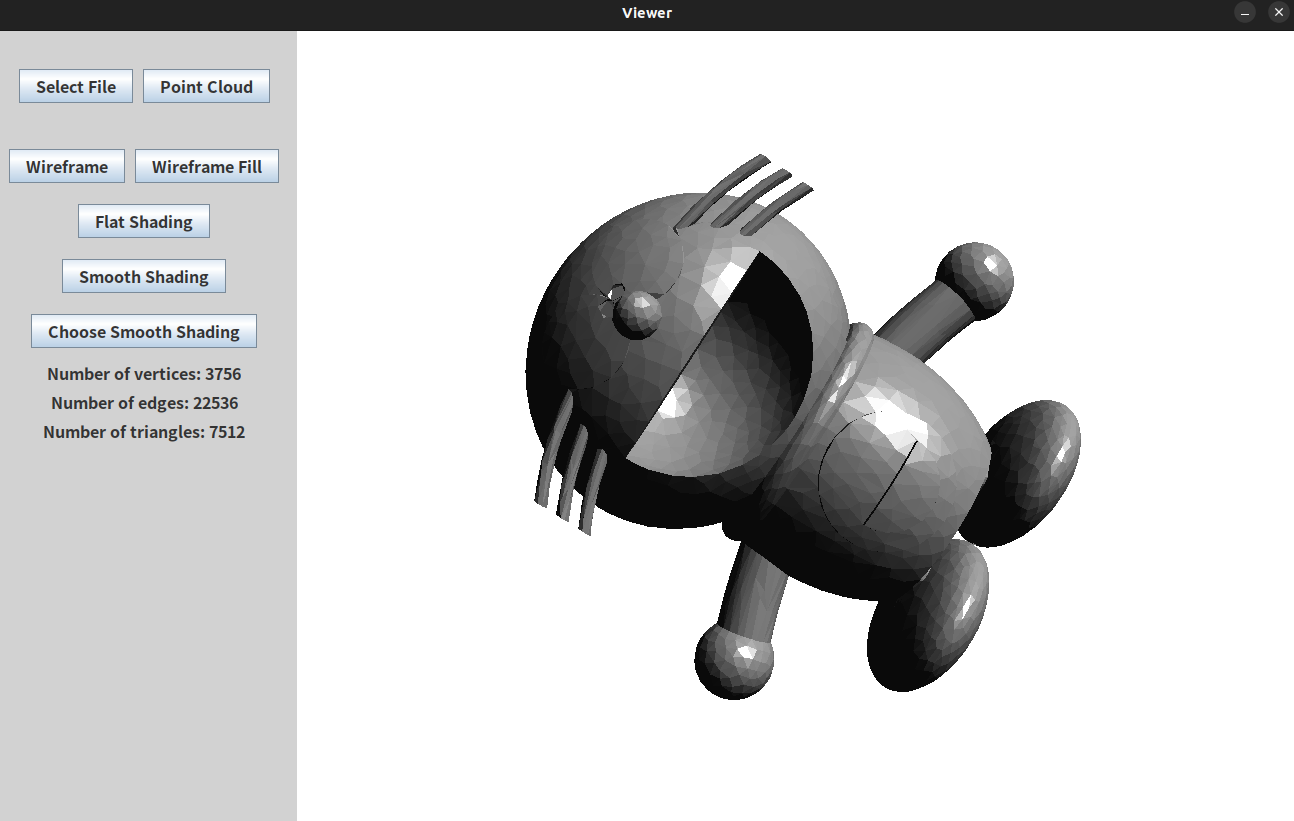
\includegraphics[width=1.0\textwidth]{sc4.png}
    \caption{Screenshot of FlatShading}
    \label{fig:my_label}
\end{figure}

\begin{figure}[h]
    \centering
    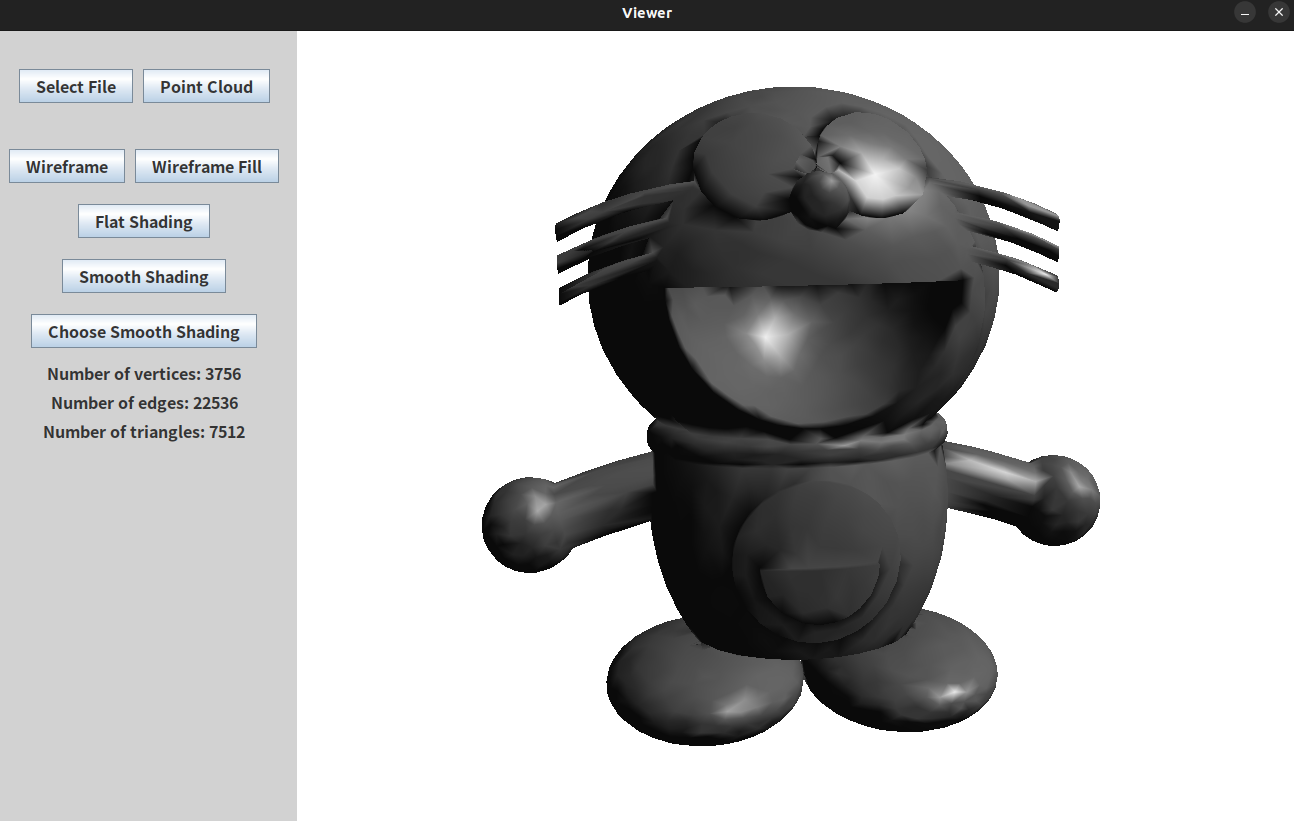
\includegraphics[width=1.0\textwidth]{sc5.png}
    \caption{Screenshot of SmoothShading}
    \label{fig:my_label}
\end{figure}

\begin{figure}[h]
    \centering
    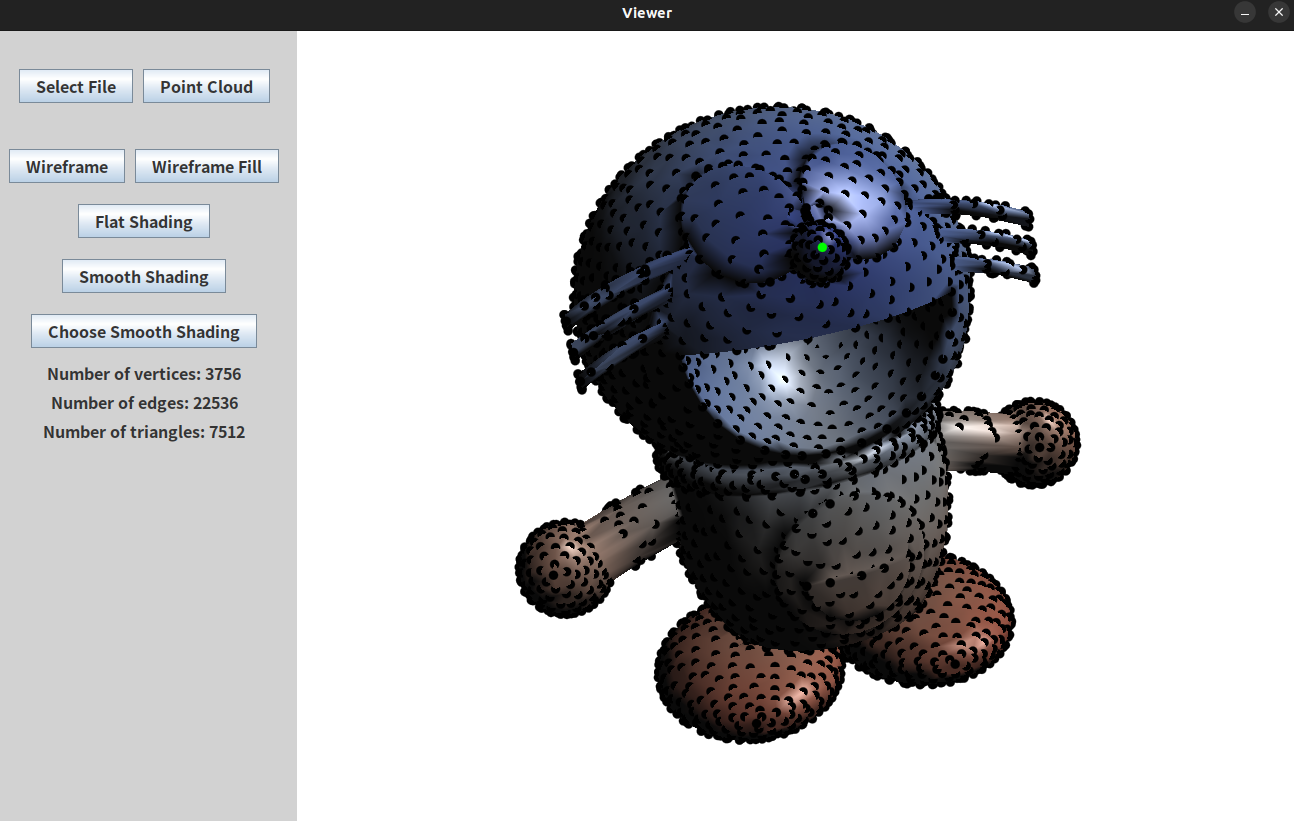
\includegraphics[width=1.0\textwidth]{sc6.png}
    \caption{Screenshot of Geodesic Distance}
    \label{fig:my_label}
\end{figure}

\end{document}
